\documentclass[../../../main.tex]{subfiles}

\begin{document}
\subsection*{Magnetized Object}
All magnetic phenomena are due to electric charges in motion, and in fact, if you could examine a piece of magnetic material on an atomic scale you would find tiny currents: electrons orbiting around nuclei and spinning about their axes--in other words, dipole. Ordinarily, they cancel each other out because of the random orientation of the atoms. But when a magnetic field is applied, a net alignment of these magnetic dipoles occurs, and the medium becomes magnetically polarized, or magnetized. 

Unlike electric polarization, which is almost always in the same direction as \textbf{E}, some materials acquire a magnetization parallel to \textbf{B} (paramagnets) and some opposite to \textbf{B} (diamagnets). A few substances, called ferromagnets, retain their magnetization even after the external field has been removed—for these, the magnetization is not determined by the present field but by the whole magnetic “history” of the object.

\subsection*{Paramagnetism and Torques}
Center the loop at the origin, and tilt it an angle $\theta$ from the $z$ axis towards the y-axis. Let \textbf{B} point in the $z$ direction. The forces on the two sloping sides cancel--they tend to stretch the loop, but they don’t rotate it. 
\begin{equation*}
    \mathbf{N} = aF \sin \theta\; \mathbf{\hat{x}}
\end{equation*}
The magnitude of the force on each of these segments is
\begin{equation*}
    F = I bB
\end{equation*}
and therefore
\begin{equation*}
    \mathbf{N} = I abB \sin \theta\; \mathbf{\hat{x}}=mB\sin\theta\;\mathbf{\hat{x}}
\end{equation*}
or
\begin{equation*}
    \mathbf{N}=\mathbf{m}\times\mathbf{B}
\end{equation*}
where $m = I ab$ is the magnetic dipole moment of the loop. 
\begin{figure*}[b]
    \centering
    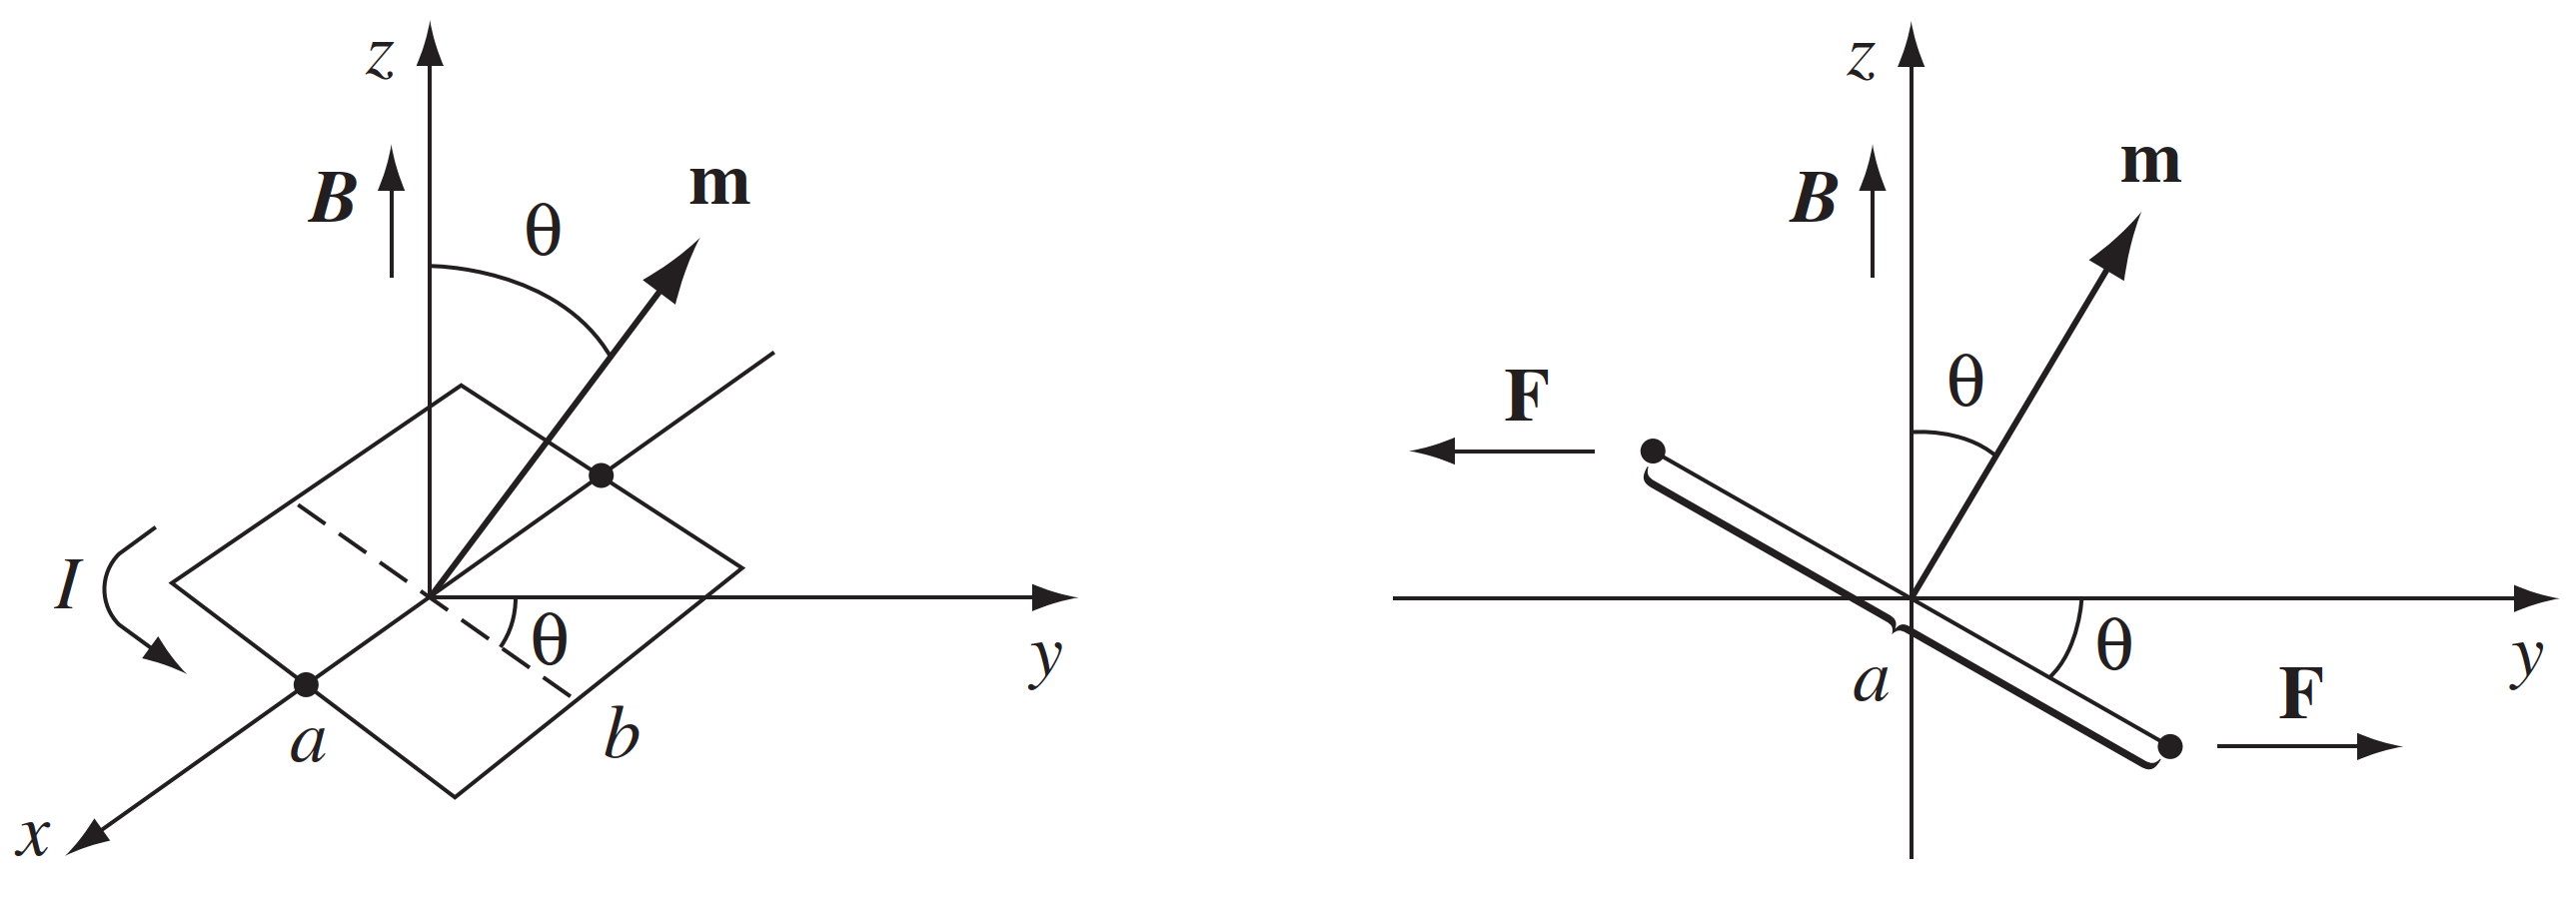
\includegraphics[width=0.8\textwidth]{../Rss/Electromagnetism/FieldInsideMatter/Torque.png}
\end{figure*}

Notice that magnetic torque $ \mathbf{N}=\mathbf{m}\times\mathbf{B}$ is identical in form to the electrical analog, $\mathbf{N} = \mathbf{p} \times \mathbf{E}$. In particular, the torque is again in such a direction as to line the dipole up parallel to the field. It is this torque that accounts for paramagnetism.

Actually, quantum mechanics tends to lock the electrons within a given atom together in pairs with opposing spins, and this effectively neutralizes the torque on the combination. As a result, paramagnetism most often occurs in atoms or molecules with an odd number of electrons. Even here, the alignment is far from complete, since random thermal collisions tend to destroy the order.

In a uniform field, the net force on a current loop is zero:
\begin{equation*}
    \mathbf{F}=I\oint (d\mathbf{l}\times \mathbf{B})=I\biggl(\oint d\mathbf{l}\biggr)\times \mathbf{B}=0
\end{equation*}
the constant \textbf{B} comes outside the integral, and the net displacement. Around a closed loop vanishes. In a nonuniform field this is no longer the case. In general, for an infinitesimal loop, with dipole moment $\mathbf{m}$, in a field \textbf{B}, the force is
\begin{equation*}
    \mathbf{F}=\nabla(\mathbf{m}\cdot\mathbf{B})
\end{equation*}

Early physicists thought magnetic dipoles consisted of positive and negative magnetic “charges” (north and south “poles,” they called them), separated by a small distance, just like electric dipoles. It’s not a bad model, but it’s bad physics, because there’s no such thing as a single magnetic north pole or south pole. Magnetism is not due to magnetic monopoles, but rather to moving electric charges; magnetic dipoles are tiny current loops.
\begin{figure*}
    \centering
    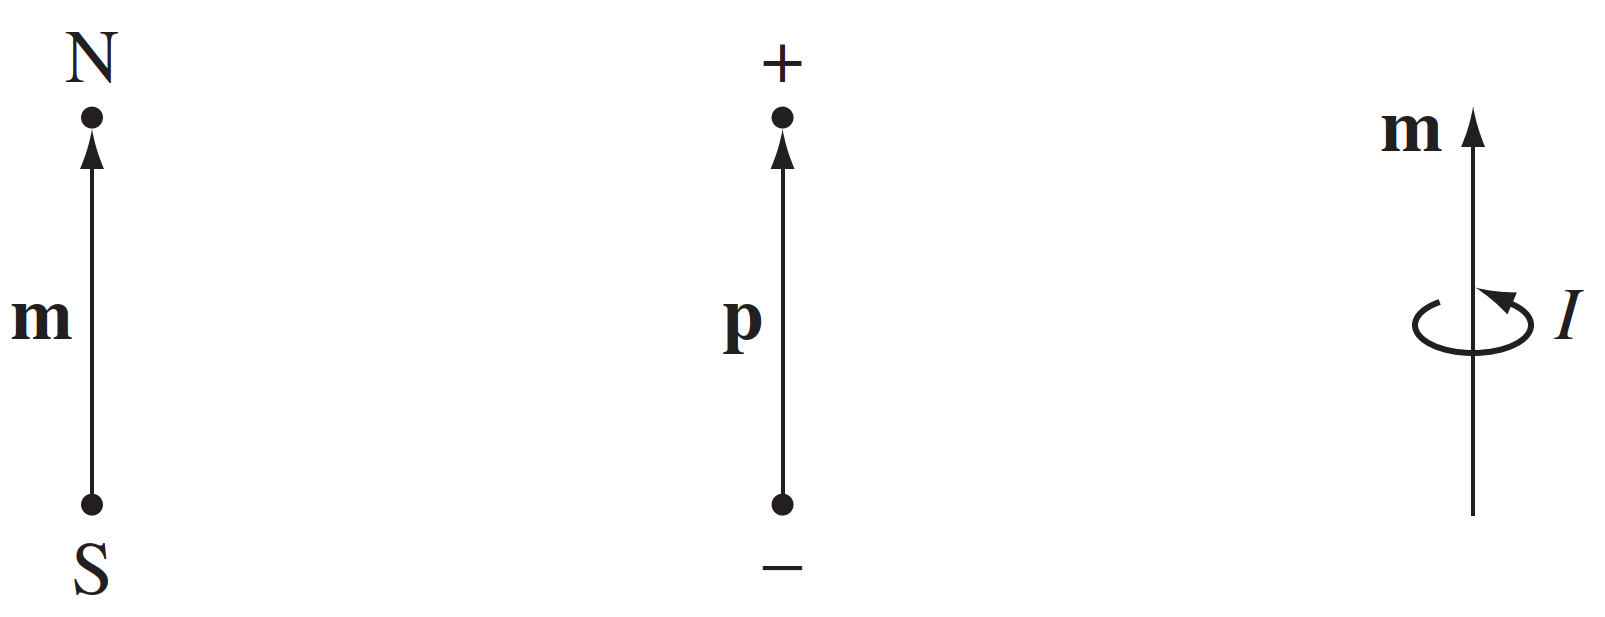
\includegraphics[width=0.5\textwidth]{../Rss/Electromagnetism/FieldInsideMatter/DipModel.png}
    \caption*{Figure: Gilbert model, electric dipole and Ampere model}
\end{figure*}

\subsection*{Diamagnetism and Electrons Orbit}
Let’s assume the  orbit of electrons is a circle of radius $R$. Although technically this orbital motion does not constitute a steady current, in practice it's going to look like a steady current with period the period $T = 2\pi R/v$
\begin{equation*}
    I=\frac{-e}{T}=-\frac{ev}{2\pi R}
\end{equation*}
Accordingly, the orbital dipole moment $(I \pi R^2)$ is
\begin{equation*}
    \mathbf{m}=-\frac{1}{2}evR \;\mathbf{\hat{z}}
\end{equation*}

\begin{figure*}[b]
    \centering
    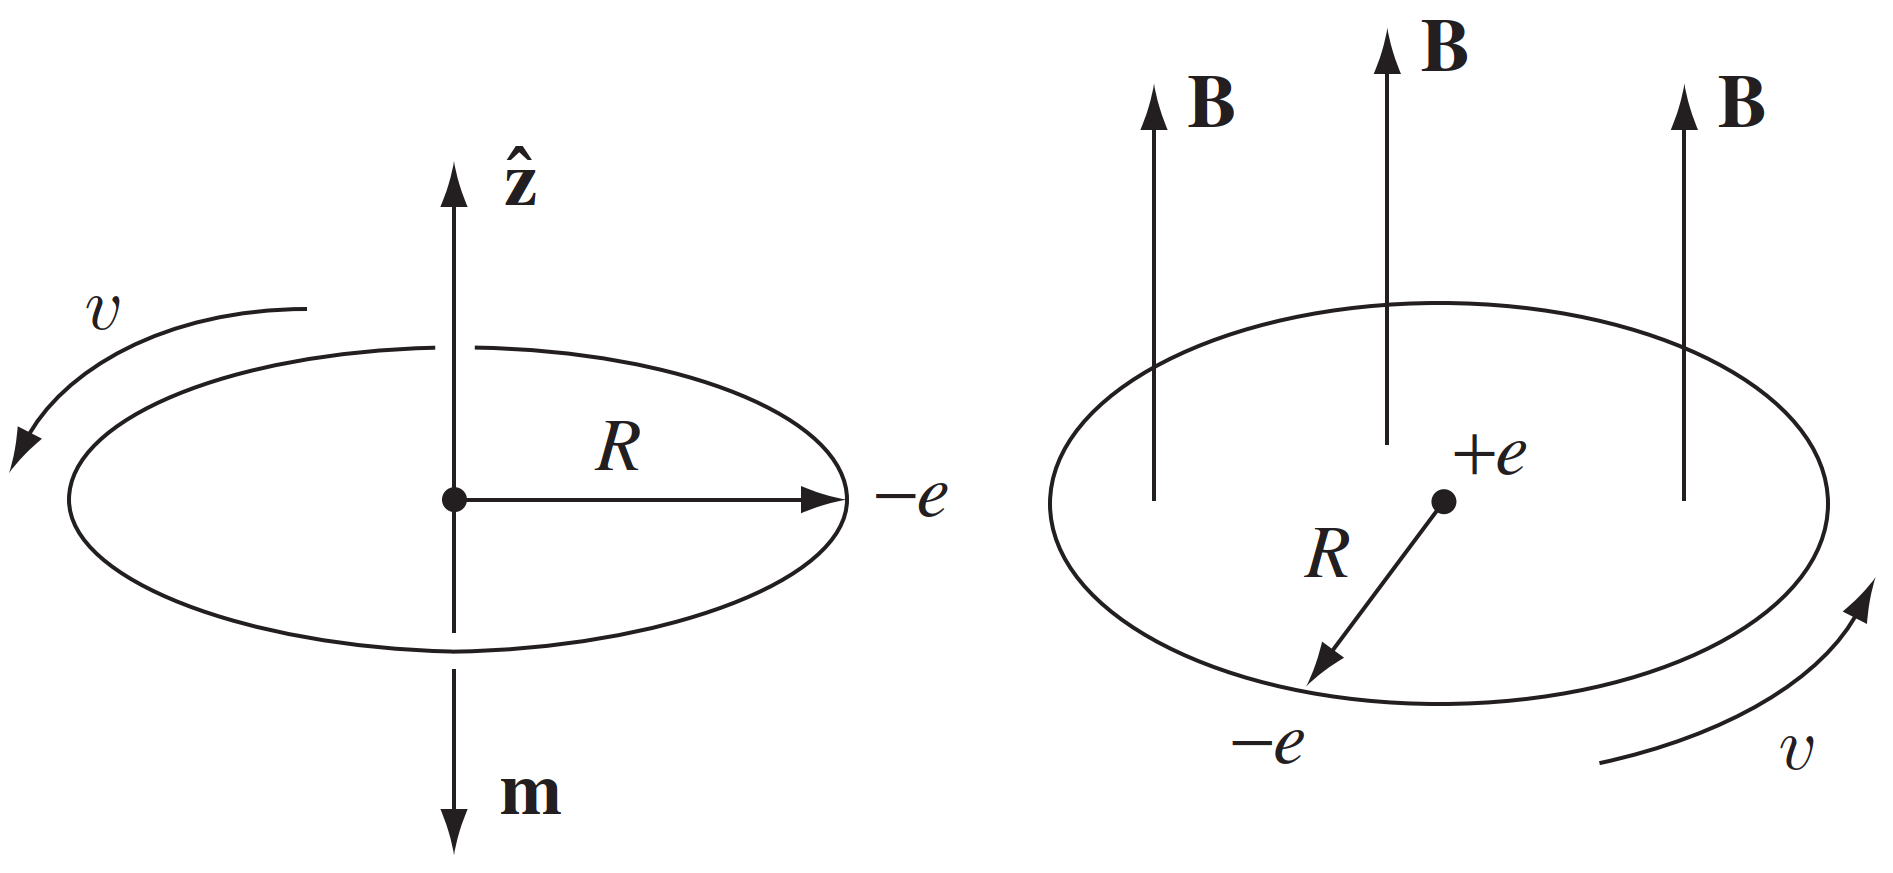
\includegraphics[width=0.7\textwidth]{../Rss/Electromagnetism/FieldInsideMatter/EOrbit.png}
    \caption*{Figure: Electron orbit before and after external field}
\end{figure*}

The centripetal acceleration $v^2/R$ is ordinarily sustained by electrical forces alone
\begin{equation*}
    -\frac{1}{4\pi \epsilon_0}\frac{e^2}{R^2}=m_e\frac{v^2}{R^2}
\end{equation*}
However, in the presence of a magnetic field there is an additional force, Lorentz's force. For the sake of argument, let's say that \textbf{B} is perpendicular to the plane of the orbit
\begin{equation*}
    -\frac{1}{4\pi \epsilon_0}\frac{e^2}{R^2}-e\bar{v}B=m_e\frac{\bar{v}^2}{R}
\end{equation*}
Under these conditions, the new speed $\bar{v}$ is greater than $v$
\begin{equation*}
    e\bar{v}B=\frac{m_e}{R}(\bar{v}^2-v^2)=\frac{m_e}{R}(\bar{v}+v)(\bar{v}-v)
\end{equation*}
or, assuming the change $\Delta v =\bar{v} - v$ is small
\begin{equation*}
    \Delta v =\frac{eRB}{2m_e}
\end{equation*}

Thus, when \textbf{B} is turned on, then, the electron speeds up. A change in orbital speed means a change in the dipole moment
\begin{equation*}
    \Delta\mathbf{m}=-\frac{1}{2}e\Delta v R \;\mathbf{\hat{z}}=-\frac{e^2R^2}{4m_e}\mathbf{B}
\end{equation*}
Notice that the change in m is opposite to the direction of \textbf{B}. Ordinarily, the electron orbits are randomly oriented, and the orbital dipole moments cancel out. But in the presence of a magnetic field, each atom picks up a little “extra” dipole moment, and these increments are all antiparallel to the field. This is the mechanism responsible for diamagnetism. It is typically much weaker than paramagnetism, and is therefore observed mainly in atoms with even numbers of electrons, where paramagnetism is usually absent.

\subsection*{Magnetization}
In the presence of a magnetic field, matter becomes magnetized. We have discussed two mechanisms that account for this magnetic polarization: (1) paramagnetism (the dipoles associated with the spins of unpaired electrons experience a torque tending to line them up parallel to the field) and (2) diamagnetism (the orbital speed of the electrons is altered in such a way as to change the orbital dipole moment in a direction opposite to the field). Whatever the cause, we describe the state of magnetic polarization by the vector quantity
\begin{equation*}
    \mathbf{M}\equiv\text{magnetic moment per unit volume}=\frac{\mathbf{m}}{\mathcal{V}}
\end{equation*}
called the magnetization. 

\subsection*{Bound Current} 
The vector potential of a single dipole \textbf{m} is
\begin{equation*}
    \mathbf{A} (\mathbf{r})=\frac{\mu_0}{4\pi}  \frac{\mathbf{m}\times \brcurs}{\rcurs^2}
\end{equation*}
In the magnetized object, each volume element $d\tau'$ carries a dipole moment $\mathbf{M} \; d\tau'$, so the total vector potential is
\begin{equation*}
    \mathbf{A} (\mathbf{r})=\frac{\mu_0}{4\pi} \int \frac{\mathbf{M}\times \brcurs}{\rcurs^2} d\tau'
\end{equation*}
That does it, in principle. But, as in the electrical case, the integral can be cast in a more illuminating form

\begin{equation*}
    \mathbf{A} (\mathbf{r})=\frac{\mu_0}{4\pi}\bigg[\int\frac{1}{\rcurs}\big(\nabla' \times \mathbf{M}(\mathbf{r'})\big)d\tau'+\oint\frac{1}{\rcurs}\big(\mathbf{M}(\mathbf{r'}) \times \big)d\mathbf{a}'\bigg] 
\end{equation*}
The first term looks just like the potential of a volume current
\begin{equation*}
    \mathbf{J}_b=\nabla \times \mathbf{M}
\end{equation*}
while the second looks like the potential of a surface current
\begin{equation*}
    \mathbf{K}_b= \mathbf{M}\times \mathbf{\hat{n}}
\end{equation*}
where $\mathbf{\hat{n}}$ is the normal unit vector. With these definitions
\begin{equation*}
    \mathbf{A} (\mathbf{r})=\frac{\mu_0}{4\pi}\bigg[\int_\mathcal{V}\frac{\mathbf{J}_b}{\rcurs} d\tau'+\oint_\mathcal{S}\frac{ \mathbf{K}_b}{\rcurs}  d\mathbf{a}' \bigg] 
\end{equation*}

What this means is that the potential (and hence also the field) of a magnetized object is the same as would be produced by a volume current throughout the material, plus a surface current on the boundary. Instead of integrating the contributions of all the infinitesimal dipoles, we first determine the bound currents, and then find the field they produce, in the same way we would calculate the field of any other volume and surface currents.

\subsubsection*{Physical interpretation.} Consider thin slab of uniformly magnetized material, with the dipoles represented by tiny current loops--notice that all the “internal” currents cancel. Say that each of the tiny loops has area $a$ and thickness $t$. In terms of the magnetization $M$, its dipole moment is $m = Mat$. In terms of the circulating current $I$, however, $m = I a$. Therefore, $I = Mt$, so the surface current is $K_b = I/t = M$, more precisely 
\begin{equation*}
    \mathbf{K}_b=\mathbf{M}\times \mathbf{\hat{n}}
\end{equation*}

When the magnetization is nonuniform, the internal currents no longer cancel. Consider two adjacent chunks of magnetized material. On the surface where they join, there is a net current in the $x$ direction, given by
\begin{equation*}
    I_x = [M_z(y + dy) - M_z(y)] dz=\frac{\partial M_z}{\partial y} dy\;dz
\end{equation*}
The corresponding volume current density is therefore
\begin{equation*}
    (J_b)_x =\frac{\partial M_z}{\partial y} 
\end{equation*}
By the same token, a nonuniform magnetization in the y direction would contribute an amount $-\partial M_y/\partial z$, so
\begin{equation*}
    (J_b)_x =\frac{\partial M_z}{\partial y} -\partial M_y/\partial z
\end{equation*}
In general, then
\begin{equation*}
    \mathbf{J}_b=\nabla \times \mathbf{M}
\end{equation*}

\subsection*{Auxiliary Field H}
the effect of magnetization is to establish bound currents $ \mathbf{J}_b=\nabla \times \mathbf{M}$ within the material and $ \mathbf{K}_b=  \mathbf{M}\times\mathbf{\hat{n}}$ on the surface. We are now ready to put everything together: the field attributable to bound currents, plus the field due to everything else--which I shall call the free current
\begin{equation*}
    \mathbf{J}=\mathbf{J}_b+\mathbf{J}_f
\end{equation*}
The free current is there because somebody hooked up a wire to a battery—it involves actual transport of charge; the bound current is there because of magnetization—it results from the conspiracy of many aligned atomic dipoles.

Ampère’s law then can be written
\begin{align*}
    \frac{1}{\mu_0}\nabla\times \mathbf{B}&=\mathbf{J}\\
    \frac{1}{\mu_0}\nabla\times \mathbf{B}&=\nabla \times \mathbf{M}+\mathbf{J}_f\\
    \mathbf{J}_f&=\nabla\times\bigg(\frac{\mathbf{B}}{\mu_0}-\mathbf{M}\bigg)
\end{align*}
The quantity in parentheses is designated by the letter \textbf{H}
\begin{equation*}
    \mathbf{H}\equiv\frac{\mathbf{B}}{\mu_0}-\mathbf{M}
\end{equation*}
In terms of \textbf{H}, then, Ampère’s law reads
\begin{equation*}
    \nabla\times\mathbf{H}=\mathbf{J}_f
\end{equation*}
or
\begin{equation*}
    \oint \mathbf{H}\cdot d\mathbf{l}=I_{\text{f}_\text{enc}}
\end{equation*}
where $I_{\text{f}_\text{enc}}$ is the total free current passing through the Amperian loop.

\subsubsection*{Deceptive parallel.} Whereas $\nabla \cdot \mathbf{B} = 0$, the divergence of \textbf{H} is not, in general, zero. In fact 
\begin{equation*}
    \nabla \cdot\mathbf{H}=-\nabla\mathbf{M}
\end{equation*}
Only when the divergence of \textbf{M} vanishes is the parallel between \textbf{B} and $\mu_0\mathbf{M}$ faithful. If the problem to find \textbf{H} exhibits cylindrical, plane, solenoidal, or toroidal symmetry, then you can get H by the usual Ampère’s law methods. If the requisite symmetry is absent, you’ll have to think of another approach, and in particular you must not assume that \textbf{H} is zero just because there is no free current in sight. 

\subsection*{Linear Medium}
In paramagnetic and diamagnetic materials, the magnetization is sustained by the field; when \textbf{B} is removed, \textbf{M} disappears. In fact, for most substances the magnetization is proportional to the field. Thus, I express the proportionality in terms of \textbf{H}, instead of \textbf{B}
\begin{equation*}
    \mathbf{M}=\chi_m \mathbf{H}
\end{equation*}
The constant of proportionality $\chi_m$ is called the magnetic susceptibility; it is a dimensionless quantity that varies from one substance to another--positive for paramagnets and negative for diamagnets.

Materials that this equation are called linear media. In terms of \textbf{B}
\begin{equation*}
    \mathbf{B} = \mu_0(\mathbf{H} + \mathbf{M}) = \mu_0(1 + \chi_m )\mathbf{H}
\end{equation*}
Thus \textbf{B} is also proportional to \textbf{H}
\begin{equation*}
    \mathbf{B}=\mu\mathbf{H}
\end{equation*}
where
\begin{equation*}
    \mu\equiv\mu_0(1 + \chi_m )
\end{equation*}
is called the permeability of the material. In a vacuum, where there is no matter to magnetize, the susceptibility $\chi_m$ vanishes, and the permeability is $\mu_0$. That’s why $\mu_0$ is called the permeability of free space. If you factor out $\mu_0$, what’s left is called the relative permeability
\begin{equation*}
    \mu_r=1 + \chi_m=\frac{\mu}{\mu_0}
\end{equation*}

Incidentally, the volume bound current density in a homogeneous linear material is proportional to the free current density
\begin{equation*}
    \mathbf{J}_b=\nabla\times \mathbf{M}=\nabla\times \chi_m \mathbf{H}=\chi_m\mathbf{J}_f
\end{equation*}

\subsubsection*{Defective parallel.} You might suppose that linear media escape the defect in the parallel between \textbf{B} and \textbf{H}: since \textbf{M} and \textbf{H} are now proportional to \textbf{B}, does it not follow that their divergence, must always vanish? Unfortunately, it does not. Formally,
\begin{align*}
    \nabla\cdot\mathbf{H}&= \nabla\cdot\frac{\mathbf{B}}{\mu}\\
    \nabla\cdot\mathbf{H}&=\frac{1}{\mu}\nabla\cdot\mathbf{B}+\mathbf{B}\cdot\nabla\cdot\frac{1}{\mu}\\
    \nabla\cdot\mathbf{H}&=\mathbf{B}\cdot\nabla\cdot\frac{1}{\mu}
\end{align*}
so \textbf{H} is not divergenceless (in general) at points where $\mu$ is changing. For instance, at the end of a cylinder of linear paramagnetic material, \textbf{M} is zero on one side but not on the other. Then 
\begin{equation*}
    \oint\mathbf{M}\neq 0
\end{equation*}
and hence, by the divergence theorem, $\nabla\cdot\mathbf{M}$ cannot vanish everywhere within it.

\subsection*{Ferromagnets}
In a linear medium, the alignment of atomic dipoles is maintained by a magnetic field imposed from the outside. Ferromagnets--which are emphatically not linear--require no external fields to sustain the magnetization; the alignment is “frozen in.” In a ferromagnet, each dipole “likes” to point in the same direction as its neighbors. The reason for this preference is essentially quantum mechanical. 

But if that is true, why isn’t every wrench and nail a powerful magnet? The answer is that the alignment occurs in relatively small patches, called domains. Each domain contains billions of dipoles, all lined up, but the domains themselves are randomly oriented and their magnetic fields cancel, so as a whole the object is not magnetized.

\subsubsection*{Hysteresis loop.} How, then, would you produce a permanent magnet? If you put a piece of iron into a strong magnetic field, the torque $\mathbf{N} = \mathbf{m} \times \mathbf{B}$ tends to align the dipoles parallel to the field. Since they like to stay parallel to their neighbors, most of the dipoles will resist this torque. However, at the boundary between two domains, there are competing neighbors, and the torque will throw its weight on the side of the domain most nearly parallel to the field. The net effect of the magnetic field, then, is to move the domain boundaries and domains parallel to the field grow. If the field is strong enough, one domain takes over entirely, and the iron is said to be saturated.

This process is not entirely reversible. When the field is switched off, there will be some return to randomly oriented domains, but it is far from complete. You now have a permanent magnet.

\begin{figure*}
    \centering
    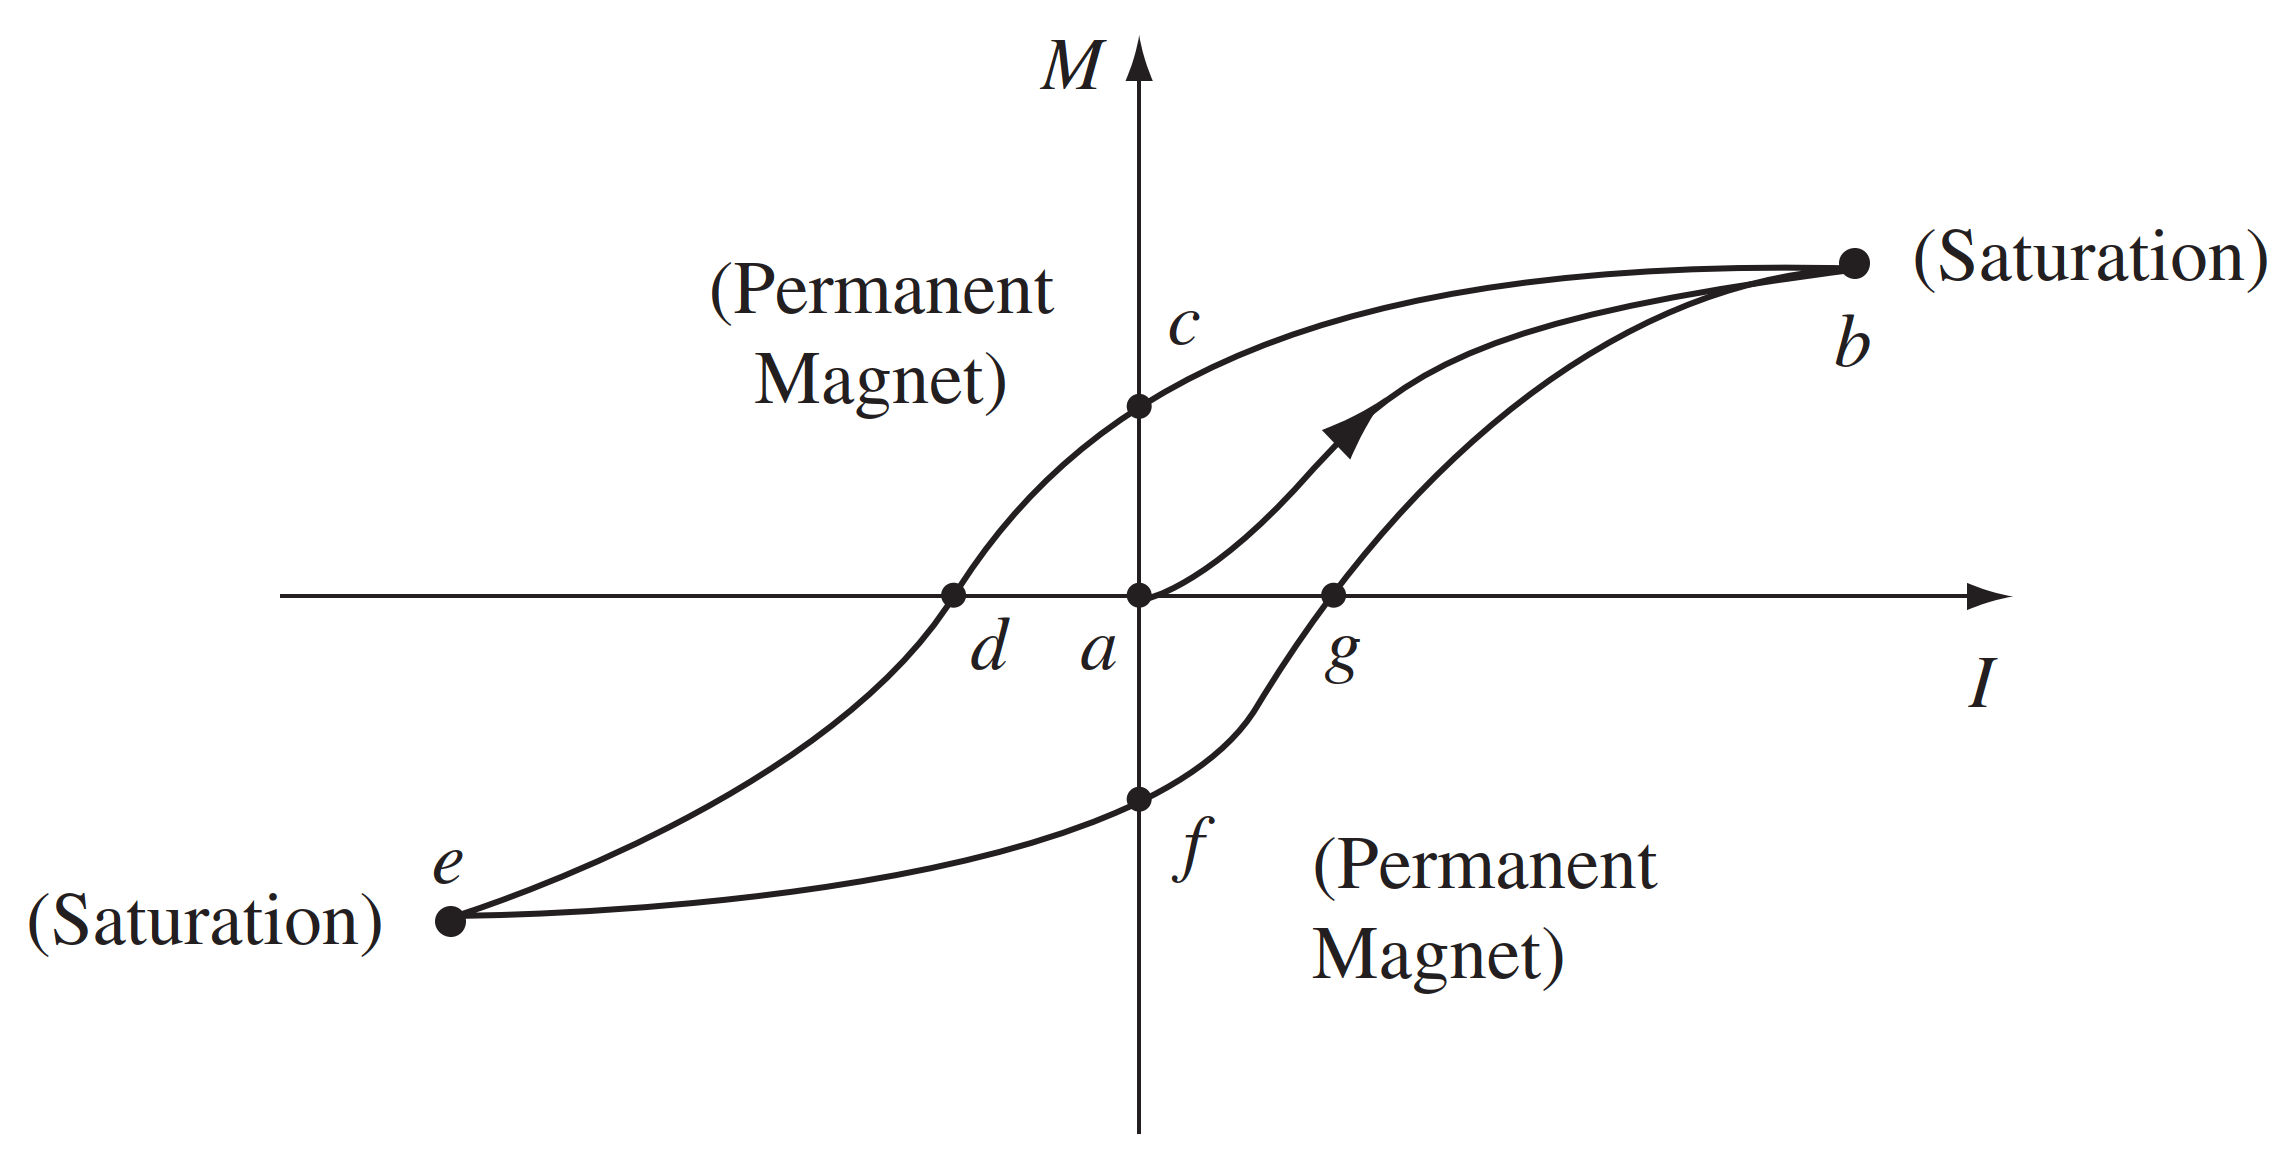
\includegraphics[width=0.75\textwidth]{../Rss/Electromagnetism/FieldInsideMatter/HysteresisLoop.png}
    \caption*{Figure: Hysteresis Loop}
\end{figure*}

A simple way to accomplish this, in practice, is to wrap a coil of wire around the object to be magnetized and run a current $I$ through the coil. As you increase the current, the field increases, the domain boundaries move, and the magnetization grows. Eventually, you reach the saturation point, with all the dipoles aligned, and a further increase in current has no effect on \textbf{M} (point $b$).

Now suppose you reduce the current. Instead of retracing the path back to $M = 0$, there is only a partial return to randomly oriented domains. $M$ decreases, but even with the current off there is some residual magnetization (point $c$). 

The object is now a permanent magnet. If you want to eliminate the remaining magnetization, you’ll have to run a current backwards through the coil (a negative $I$). As you increase $I$ (negatively), $M$ drops down to zero (point $d$). 

If you turn I still higher, you soon reach saturation in the other direction (point $e$). At this stage, switching off the current will leave the object with a permanent magnetization to the other direction (point $f$). To complete the story, turn $I$ on again in the positive sense: M returns to zero (point $g$), and eventually to the forward saturation point (point $b$).

Notice that the magnetization of the object depends not only on the applied field (that is, on $I$), but also on its previous magnetic “history.” It is customary to draw hysteresis loops as plots of $B$ against $H$, rather than $M$ against $I$. If our coil is approximated by a long solenoid, with $n$ turns per unit length, then $H = nI $, so $H$ and $I$ are proportional. Meanwhile, $\mathbf{B} = \mu_0(\mathbf{H} + \mathbf{M})$, but in practice $M$ is huge compared to $H$, so to all intents and purposes $B$ is proportional to $M$.

To make the units consistent (Tesla), I have plotted ($\mu_0 H$) horizontally; notice, however, that the vertical scale is $10^4$ times greater than the horizontal one. Roughly speaking, $\mu\mathbf{H}$ is the field our coil would have produced in the absence of any iron; B is what we actually got. That’s why anyone who wants to make a powerful electromagnet will wrap the coil around an iron core. It doesn’t take much of an external field to move the domain boundaries, and when you do that, you have all the dipoles in the iron working with you.

\begin{figure*}
    \centering
    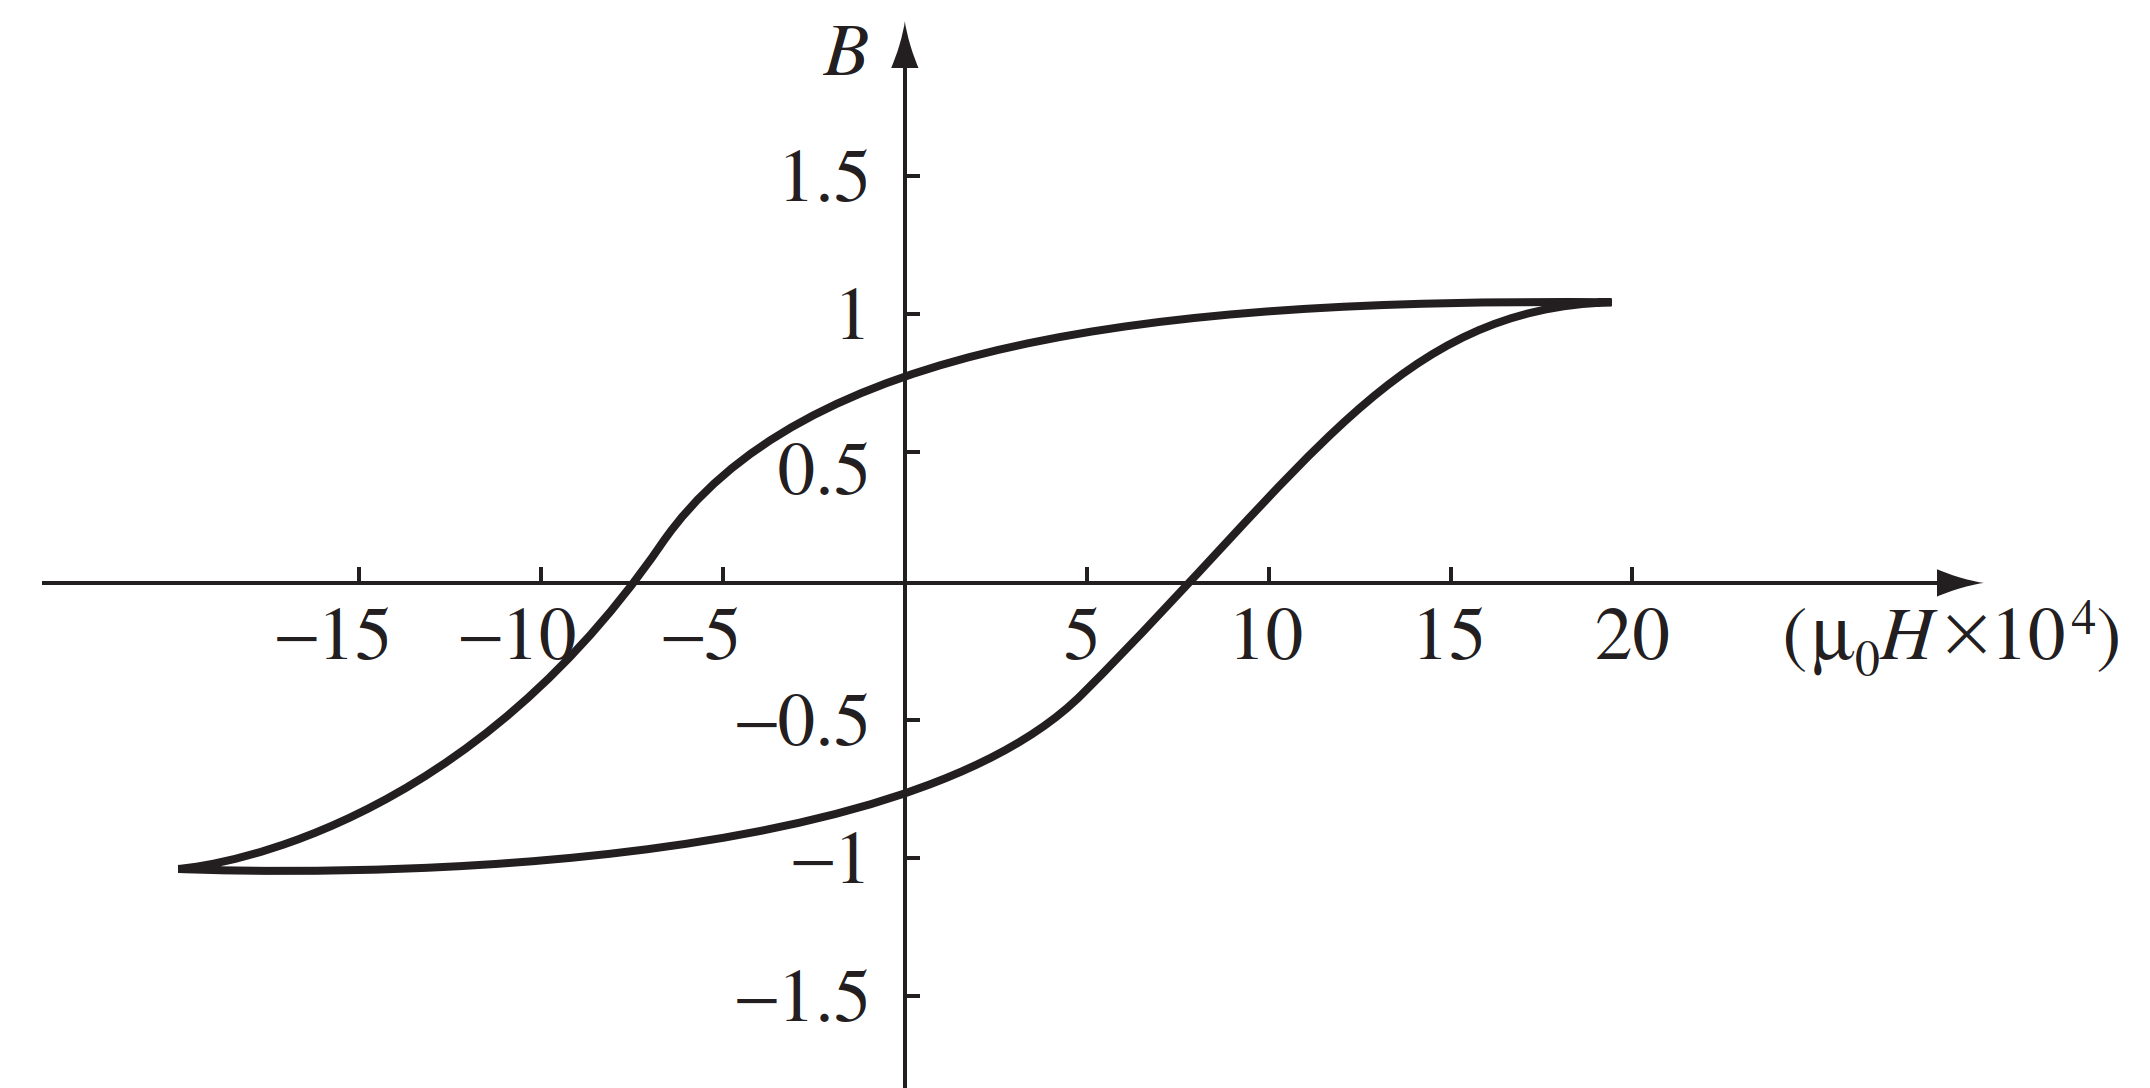
\includegraphics[width=0.75\textwidth]{../Rss/Electromagnetism/FieldInsideMatter/HysteresisLoop2.png}
    \caption*{Figure: Hysteresis Loop}
\end{figure*}
One final point about ferromagnetism: It all follows, remember, from the fact that the dipoles within a given domain line up parallel to one another. Random thermal motions compete with this ordering, but as long as the temperature doesn’t get too high, they cannot budge the dipoles out of line. It’s not surprising, though, that very high temperatures do destroy the alignment. What is surprising is that this occurs at a precise temperature, called the Curie point.
\end{document}